\chapter{Analyse}
\label{chapter:analyse}

In Kapitel \ref{chapter:grundlagen} wurden für die weitere Betrachtung der Streaming frameworks notwendige Grundbegriffe erläutert und ein Referenzmodell wie in Abbildung \ref{fig:basismodell} gezeigt vorgestellt. Zunächst wird der Markt anhand der Studie \citelit{studie:bidama} im Kontext von Big Data in dem Streaming frameworks zum Einsatz kommt vorgestellt. Die Studie \citelit{studie:bidama} wurde von Markl et al. im Auftrag des Bundesministeriums für Wirtschaft und Energie (BMWi) 2013 erstellt. 

\begin{quote}
Zentrales Ziel der vorliegenden Studie ist eine qualitative und quantitative Bewertung des Ist-Zustandes sowie der wirtschaftlichen Potenziale von neuen Technologien für das Management von Big Data. Daraus werden standortspezifische Chancen und Herausforderungen für Deutschland abgeleitet. In der Studie werden insbesondere auch rechtliche Rahmenbedingungen anhand von Einzelfällen betrachtet. Die Studie beinhaltet zudem konkrete Handlungsempfehlungen. 
\citelit[S. 3]{studie:bidama}
\end{quote}

Big Data wurde im Artikel \citelit{laney:threevs} von Laney 2001 in drei Dimensionen \textit{volume}, \textit{velocity} und \textit{variety} eingeordnet. Die Dimension \textit{volume} beschreibt den Umgang mit dem rasanten Anstieg an Datentransaktionen. \textit{Velocity} gibt die Geschwindigkeit an und \textit{variety} gibt die steigende Vielfalt der Daten an. In der Abbildung \ref{fig:bigdatacube} werden die drei Dimensionen in einem Würfel dem \textit{Big Data Cube} dargestellt. Die Abbildung \ref{fig:bigdatacube} wurde aus \citelit[S. 1, Abb. 1]{meijer2012your} in einfacher Form übernommen. So beschreibt Meijer \textit{volume} von klein \textit{small} nach groß \textit{big}, \textit{velocity} von ziehen \textit{pull} nach drücken \textit{push} und \textit{variety} von komplexen strukturierten Daten Fremd-/Primärschlüssel \textit{\acrshort{glo:fk}/\acrshort{glo:pk}} nach einfachen Zeigern auf Daten und Daten \textit{\acrshort{glo:k}/\acrshort{glo:v}}. Das herkömmliche relationale Datenbanksystem ist in der Abbildung \ref{fig:bigdatacube} unter den Koordinaten (\textit{small}, \textit{pull}, \textit{fk/pk}) zu finden. Unter den Koordinaten (\textit{small}, \textit{pull}, \textit{k/v}) wären Anwendungen zu finden, die das Konzept \textit{\gls{glo:orm}} implementieren. Beim Konzept \textit{\gls{glo:orm}} werden Objekte in relationalen Datenbanken abgebildet \citelit[S. 1]{meijer2012your}. Die Streaming frameworks werden unter den Koordinaten (\textit{big}, \textit{push}, \textit{fk/pk}) eingeordnet. Gegenüber den Streaming frameworks unter den Koordinaten (\textit{big}, \textit{pull}, \textit{fk/pk}) befinden sich die Batch Processing Engines, wie zum Beispiel Apache Hadoop \citeint{res:apache:hadoop}. In der unteren linken Ecke (big, pull, k/v) werden Lambda Ausdrücke eingeordnet. Lambda Ausdrücken werden anonyme Methoden möglich. Damit können einfache Abfragen auf Sammlungen formalisiert werden. Der Compiler erzeugt zur Laufzeit die Methoden im Hintergrund. In Java stehen die Lambda Ausdrücke erst ab Version 8 zur Verfügung \citeint{res:oracle:java8}.

\begin{figure}[htb!]
\centering
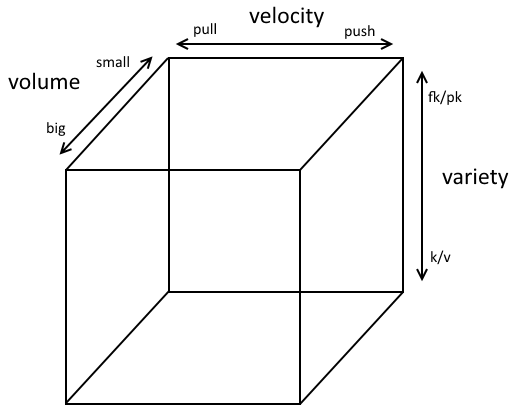
\includegraphics[width=1.0\textwidth]{bilder/bigdatacube.png}
\caption{Darstellung Big Data Cube
\label{fig:bigdatacube}}
\end{figure}

Relationale Datenbanksysteme stoßen im Zusammenhang der horizontalen Skalierung in der zentralisierten Systemarchitektur auf Probleme, wenn die Datenmenge die Kapazität einer Maschine übersteigt und dadurch das Ergebnis in keiner akzeptablen Zeit zurückgegeben wird \citelit[S. 30, Kap. 2.2.1]{edlich:nosql}. So zeigt Edlich et al. in dem Buch \citelit{edlich:nosql} einen alternativen Ansatz Daten zu halten. Dabei wird der Begriff \textit{NoSQL} als nicht relationales Datenbanksystem eingeführt und definiert \citelit[S. 2, K 1.2]{edlich:nosql}. In Verbindung mit horizontaler Skalierung, Replikation und niedriger Reaktionszeit wird in \citelit[S. 30, K. 2.2]{edlich:nosql} das \gls{glo:cap}-Theorem erklärt. Beim CAP-Theorem besteht der Konflikt in der Konsistenz \textit{C}. Es gilt zu Entscheiden ob die Konsistenz gelockert wird oder nicht. Bei einer lockeren Konsistenz und damit einer hohen Verfügbarkeit und Ausfalltoleranz können in einem Verbindungsausfall alte Zustände zurückgegeben werden. Falls nicht gelockert wird kann der Umstand in Kraft treten, sehr lange Reaktionszeiten zu erhalten. %Out-of-order, Dropped, Duplicate Messages
Daher wurde das Konsistenzmodell \gls{glo:base} eingeführt. Es basiert auf einem optimistischen Ansatz. Eine Transaktion nimmt den Status konsistent nicht unmittelbar ein. Erst nach einer gewissen Zeitspanne ist die Transaktion konsistent. Dieses Verhalten wird als \textit{Eventually Consistancy} bezeichnet. Als Beispiel gibt Edlich et al. in \citelit[S. 33, K. 2.2.3]{edlich:nosql} replizierende Knoten in einer Systemarchitektur an. 
% 3V Darstellung, nächere Darstellung ACID(::CAP)->BASE %% --> CRDTs

So wurden in der Studie \citelit{studie:bidama} neben der Einführung in Big Data, Stärken, Schwächen, Chancen und Risiken für die Branchen Handel, Banken, Energie, Dienstleistungen, Öffentlicher Sektor, Industrie, Gesundheitssektor, Marktforschung, Mobilitätsleistungen, Energie und Versicherungen als tabellarische Übersicht in \citelit[S. 105, Tab. 18]{studie:bidama} ausgegeben. In \citelit[S. 107, Abb. 54]{studie:bidama} werden Branchenschwerpunkte abgeleitet. Die genannte Abbildung wird im folgenden Zitat textuell erneut wiedergegeben:

\begin{quote}
	\begin{enumerate}
		\item Entwicklung neuartiger Technologien, um eine skalierbare Verarbeitung von komplexen Datenanalyseverfahren auf riesigen, heterogenen Datenmengen mit hoher Datenrate zu realisieren
		\item Senkung der Zeit und Kosten der Datenanalyse durch automatische Parallelisierung und Optimierung von deklarativen Datenanalysespezifikationen
		\item Schaffung von Technologieimpulsen, die zur erfolgreichen weltweiten Kommerzialisierung von in Deutschland entwickelten, skalierbaren Datenanalysesystemen führen
		\item Ausbildung von Multiplikatoren im Bereich der Datenanalyse und der skalierbaren Datenverarbeitung, welche die Möglichkeiten von Big Data in Wissenschaft und Wirtschaft tragen werden
		\item Technologietransfer an Pilotanwendungen in Wissenschaft und Wirtschaft
		\item Schaffung eines Innovationsklimas durch Konzentration von kritischem Big Data Know-how, damit deutsche Unternehmen und Wissenschaft nicht im Schatten des Silicon Valleys stehen
		\item Interaktive, iterative Informationsanalyse für Text und Weiterentwicklung geeigneter Geschäftsmodelle zur Schaffung von Marktplätzen für Daten, Datenqualität und Verwertung von Daten
		\item Datenschutz und Datensicherheit
	\end{enumerate}
	\citelit[S. 107, Abb. 54]{studie:bidama}
\end{quote}

Aus den abgeleiteten Schwerpunkten können mehrere Kriterien für die Betrachtung der Streaming frameworks in Kapitel \ref{chapter:vorstellung} und des Referenzmodells in Kapitel \ref{section:technologie} herangezogen werden. Zunächst werden die gewonnen Kriterien in einer Liste aufgezählt. Anschließend werden die einzelnen Kriterien als Bewertungskriterien für die weitere Untersuchung der Streaming frameworks definiert. Daraufhin werden die Bewertungskriterien auf das Referenzmodell angewendet.

\begin{itemlist}{Bewertungskriterien}{liste:bewkrit}
	\item Architektur
	\item Prozesse und Threads
	\item Kommunikation
	\item Namenssystem
	\item Synchronisierung
	\item Konsistenz und Replikation
	\item Pipelining und Materialisierung
	\item Fehlertoleranz
	\item Sicherheit	
\end{itemlist}

Die ermittelten Bewertungskriterien aus Liste \ref{liste:bewkrit} unterstützen die Feststellung eines Streaming frameworks und des Referenzmodells. Damit die einzelnen Bewertungskriterien bei der Anwendung eindeutig und klar sind, werden diese zunächst definiert und zusätzlich erläutert.

\begin{description}
	\item[Architektur] stellt den verwendeten Architekturstil vor und ordnet in eine Systemarchitektur ein.
	\item[Prozesse und Threads] zeigen die Anwendung von blockierendem oder nicht blockierendem Zugriff, also einer Verbindung zwischen Client und einem Server. Während der Betrachtung wird der Einsatz der verteilten Verarbeitung in der eingesetzten Architektur geprüft.
	\item[Kommunikation] gibt die Form des Nachrichtenaustauschs zwischen Client und Servern an. Zum Austausch der Nachrichten kommen Nachrichtenprotokolle zum Einsatz. Dabei wird auf die Protokollschicht Middleware-Protokoll eingegangen. Im \acrshort{glo:osi}-Modell entspricht die Sitzungs- und Darstellungsschicht der Middleware-Schicht \citelit[S. 148, Abb. 4.3 angepasstes Referenzmodell]{tanenbaum:vs}. Dabei werden unterschiedliche Strategien \gls{glo:rpc}, Warteschlangensysteme, Kontinuierliche Systeme und Multicast Systeme, die beim Nachrichtenaustauschs eingesetzt werden, innerhalb der Middleware-Protokolle eingeordnet. Außerdem wird das Verbindungsmodell, die Nachrichtenstruktur und der Einsatz einer Protokollversionierung vorgestellt. Weiterhin wird die Unterstützung von unterschiedlichen Nachrichtenkodierungen und Statusverwaltung betrachtet.
	\item[Namenssystem] zeichnet den Ansatz eines Benennungssystems. Hierbei wird linear-, hierarchisch- oder attributbasiert klassifiziert.
	\item[Synchronisierung] beschreibt die verwendeten Algorithmenarten. 
	\item[Konsistenz und Replikation] zeigt die Skalierungstechnik auf und stellt die Verwaltung der Replikation vor. 
	\item[Pipelining und Materialisierung] gibt eine Technik an, ob komplexe Aggregate berechnet werden und innerhalb der Abfragen wieder benutzt werden können.
	\item[Fehlertoleranz] zeigt das verwendete Fehlermodell und stellt eine Strategie im Wiederherstellungsfall vor.
	\item[Sicherheit] stellt das Konzept vor und beschreibt den Einsatz von sicheren Kanälen und der Zugriffssteuerung.
	\item[Qualität] beschreibt das verwendete Modell für die Dienstgüte
	\item[Erweiterung] beschreibt Methoden weitere Systemarchitekturen anzuschließen.
\end{description}

In der Liste \ref{liste:bewkrit} wurden Bewertungskriterien vorgestellt und definiert, die nun auf das Referenzmodell aus Kapitel \ref{section:technologie} angewendet werden. Formal wird zuerst eine tabellarische Übersicht gezeigt, auf die anschließend in der Erläuterung Bezug genommen wird.
%Top-K, Count-Min Sketches -> Hash Kernels

